\documentclass[11pt,a4j]{article}

% import packages
\usepackage[dvipdfmx]{graphicx}
\usepackage{authblk}
\usepackage{amsmath}
\usepackage{amssymb}
\usepackage{amsfonts}
\newtheorem{dfn}{定義}
\newtheorem{thm}{定理}
\newtheorem{lem}{補題}
\newtheorem{exm}{例}

% define new command 
\newcommand{\indep}{\mathop{\perp\!\!\!\perp}}
\newcommand{\notindep}{\mathop{\perp\!\!\!\!\!\!/\!\!\!\!\!\!\perp}}
 
% Title
\title{Kernel VAE: Gaussian Process Latent Variable Model on Deep Neural Network}
\date{2019/10/11}
\author[1]{Yuma Uchiumi\thanks{uchiumi@ailab.ics.keio.ac.jp}}
\affil[1]{Department of Information and Computer Science, Faculty of Science and Technology, Keio University, Japan}

\begin{document}
  % Title
  \maketitle
  
  % Abstract
  \begin{abstract}
    ...
  \end{abstract}

  % Contents
  \tableofcontents

  \section{Introduction}
    ...
  \section{ガウス過程と確率モデル}
    \subsection{ガウス分布}
    \paragraph{分布の再生性}
      任意の$n \in \mathbb{N}$と${\{ a_i, b_i \in \mathbb{R} \}}_{i=1}^{n}$に対して,次が成り立つ.
      \begin{align}
        &X_i \sim i.i.d. ~ \mathcal{N}(\mu_i, \sigma_i^2), ~~~ (i=1,\dots,n) \\
        &\Rightarrow \sum_{i=1}^{n} a_i X_i + b_i \sim \mathcal{N} \left( \sum_{i=1}^{n} a_i \mu_i + b_i, \sum_{i=1}^{n} a_i^2 \sigma_i^2 \right)
      \end{align}

      \paragraph{条件つき分布の計算}
      任意の2つのベクトル${\bf f}_n \in \mathbb{R}^{n}, {\bf f}_m \in \mathbb{R}^{m}$に対して,
      \begin{align}
        \left(
          \begin{array}{c}
            {\bf f}_n \\ {\bf f}_m
          \end{array}
        \right)
        \sim
        \mathcal{N} 
        \left(
          \left(
            \begin{array}{c}
              {\boldsymbol \mu}_n \\ {\boldsymbol \mu}_m
            \end{array}
          \right)
          ,
          \begin{bmatrix}
            \Sigma_{nn} & \Sigma_{nm} \\
            \Sigma_{nm}^{\mathrm{T}} & \Sigma_{mm}
          \end{bmatrix}o
        \right)
      \end{align}
      ならば,次が成り立つ.
      \begin{align}
        {\bf f}_m | {\bf f}_n \sim \mathcal{N}\left( {\boldsymbol \mu}_{m|n}, \Sigma_{m|n} \right) \label{form:gaussian_conditional}  
      \end{align}
      \begin{align}          
        where ~ 
        \begin{cases}
          {\boldsymbol \mu}_{m|n} = {\boldsymbol \mu}_{m} + \Sigma_{nm}^{\mathrm{T}} \Sigma_{nn}^{-1} ( {\bf f}_n - {\boldsymbol \mu}_{n} ) \\
          \Sigma_{m|n} = \Sigma_{mm} - \Sigma_{nm}^{\mathrm{T}} \Sigma_{nn}^{-1} \Sigma_{nm}
        \end{cases} \nonumber
      \end{align}

    \subsection{ガウス過程(GP)}
      入力空間$\mathcal{X}$上の関数$f: \mathcal{X} \to \mathbb{R}$がガウス過程(Gaussian Process, GP)に従うとは,$\mathcal{X}$上の任意の$n$点${ \{ x_i \} }_{i=1}^{n}$に対して,
      ベクトル${\bf f} = { ( f(x_1),\dots,f(x_n) ) }^{\mathrm{T}} \in \mathbb{R}^{n}$が$n$次元ガウス分布に従うことをいう.
      ここで,確率変数${\bf f} \in \mathbb{R}^{n}$が$n$次元ガウス分布に従う時,その確率密度関数$p({\bf f})$は,平均関数${m}(\cdot)$と共分散関数$v(\cdot,\cdot)$を用いて
      \begin{align}
        p({\bf f}) = \frac{1}{ {(2 \pi)}^{n/2} {| V({\bf f}) |}^{1/2} } \exp \left( {- \frac{1}{2}} {({\bf f} - m(\bf f))}^{\mathrm{T}} {V({\bf f})}^{-1} ({\bf f} - m(\bf f)) \right)
      \end{align}
      と定められる.ただし,$V({\bf f})$は共分散$v({\bf f}_i, {\bf f}_j)$を$ij$要素にもつ共分散行列である.
      ゆえに,関数$f: \mathcal{X} \to \mathbb{R}$がガウス過程(Gaussian Process, GP)に従うとき,その挙動は平均関数${m}(\cdot)$と共分散関数$v(\cdot,\cdot)$によって定められ,これを以下のように記述する.
      \begin{align}
        f(\cdot) \sim \mathcal{GP}(m(\cdot), v(\cdot,\cdot))
      \end{align}    

    \subsection{ガウス過程回帰(GPR)}
      確率変数$X \in \mathbb{R}^{d}, Y \in \mathbb{R}$の実現値からなる$n$個のデータサンプル$\mathcal{D} = {\{ {\bf x}_i, y_i \}}_{i=1}^n$
      を用いて,$X$の値から$Y$の値を推定するモデル$f:X \to Y$を特定することを回帰問題という.
      すべての$({\bf x}, y)$に対して,モデルの出力値$f({\bf x})$と$y$との誤差を$\varepsilon$とおき,これが正規分布$\mathcal{N}(0, \sigma^2)$に従うと仮定すると回帰モデルは.
      \begin{align}
        y = f({\bf x}) + \varepsilon, ~~~ \varepsilon \sim \mathcal{N}(0, \sigma^2)
      \end{align}
      あるいは,正規分布の再生性より,
      \begin{align}
        y | {\bf x} \sim \mathcal{N}(f({\bf x}), \sigma^2) \label{form:reg_likelihood}
      \end{align}
      となる.
      また一般の回帰問題において,データサンプル$\mathcal{D} = {\{ X_i, Y_i \}}_{i=1}^n$とモデル$f:X \to Y$に対して下式が成り立つことから,これはモデル$f$の分布に関するベイズ推論へ拡張できる.
      \begin{align}
        p(f|\mathcal{D}) = \frac{p(\mathcal{D}|f)p(f)}{p(\mathcal{D})}, ~~i.e.~~~
        p(f | Y,X) = \frac{ p( Y | X, f) p(f) }{p( Y | X )} \label{form:reg_bayes}
      \end{align}
      上のモデルにおいて,関数$f$がガウス過程に従う場合,これをガウス過程回帰という.
      たとえば,関数$f$に対して,
      \begin{align}
        f(\cdot) \sim \mathcal{GP}(m(\cdot), k(\cdot,\cdot)) \label{form:gp_prior}
      \end{align}
      を仮定すると,${\bf f}_n = { ( f({\bf x}_1),\dots,f({\bf x}_n) ) }^{\mathrm{T}}$と${\bf y}_n = {( y_1,\dots,y_n )}^{\mathrm{T}}$に対して,
      \begin{align}
        {\bf f}_n &\sim \mathcal{N}(m(X_n), K(X_n,X_n)) \\
        {\bf y}_n &\sim \mathcal{N}(m(X_n), K(X_n,X_n) + \sigma^2 I_n)
      \end{align}
      が成り立つ.ただし,$ m(X_n) = { ( m({\bf x}_1), \dots, m({\bf x}_n) ) }^{\mathrm{T}} $,
      $K(X_n,K(X_n))_{ij} = k(f({\bf x}_i), f({\bf x}_j))$,$I_n$は$n \times n$の単位行列とする.
      式(\ref{form:gp_prior})は,式(\ref{form:reg_bayes})でモデル$f$の事前分布$p(f)$を定めることに対応する.
      さらに,式(\ref{form:reg_likelihood})と正規分布の共役性より,ガウス過程回帰では,事前分布$p(f)$と事後分布$p(f|Y,X)$が共に正規分布に従うため,
      データサンプル$\mathcal{D} = {\{ X_i, Y_i \}}_{i=1}^n$に基づく平均関数$m(\cdot)$と共分散関数$k(\cdot,\cdot)$の行列計算($O(n^2)$)のみで事後分布の形状が求められる.
      
      さらに,未知の$m$個のデータ${\{ {\bf x}_i \} }_{i=n+1}^{n+m}$に対して,対応する${\{ y_i \} }_{i=n+1}^{n+m}$の同時分布(予測分布)を求めることもできる.
      式(\ref{form:gp_prior})より,
      \begin{align}
        \left(
          \begin{array}{c}
            {\bf f}_n \\ {\bf f}_m
          \end{array}
        \right)
        \sim
        \mathcal{N} 
        \left(
          \left(
            \begin{array}{c}
              m(X_n) \\ m(X_m)
            \end{array}
          \right)
          ,
          \begin{bmatrix}
            K(X_n,X_n) & K(X_n,X_m) \\
            {K(X_n,X_m)}^{\mathrm{T}} & K(X_m,X_m)
          \end{bmatrix}
        \right)
      \end{align}
      が成り立つから,式(\ref{form:gaussian_conditional})より,${\bf f}_m$の${\bf f}_n$に対する予測分布は,
      \begin{align}
        {\bf f}_m | {\bf f}_n \sim \mathcal{N}\left( E[{\bf f}_m | {\bf f}_n], V[{\bf f}_m | {\bf f}_n] \right) 
      \end{align}
      \begin{align}          
        where ~ 
        \begin{cases}
          E[{\bf f}_m | {\bf f}_n] = m(X_m) + {K(X_n,X_m)}^{\mathrm{T}} {K(X_n,X_n)}^{-1} ( {\bf f}_n - m(X_n) ) \\
          V[{\bf f}_m | {\bf f}_n] = K(X_m,X_m) - {K(X_n,X_m)}^{\mathrm{T}} {K(X_n,X_n)}^{-1} K(X_n,X_m)
        \end{cases} \nonumber
      \end{align}
      となり,${\bf f}_m$の${\bf y}_n$に対する予測分布は,
      \begin{align}
        {\bf f}_m | {\bf y}_n \sim \mathcal{N}\left( E[{\bf f}_m | {\bf y}_n], V[{\bf f}_m | {\bf y}_n] \right) 
      \end{align}
      \begin{align}          
        where ~ 
        \begin{cases}
          E[{\bf f}_m | {\bf y}_n] = m(X_m) + {K(X_n,X_m)}^{\mathrm{T}} {( K(X_n,X_n) + \sigma^2 I_n )} ^{-1} ( {\bf y}_n - m(X_n) ) \\
          V[{\bf f}_m | {\bf y}_n] = K(X_m,X_m) - {K(X_n,X_m)}^{\mathrm{T}} { ( K(X_n,X_n) + \sigma^2 I_n ) }^{-1} K(X_n,X_m)
        \end{cases} \nonumber
      \end{align}
      となる.よって,${\bf y}_m$の${\bf y}_n$に対する予測分布は,
      \begin{align}
        {\bf y}_m | {\bf y}_n \sim \mathcal{N}\left( E[{\bf y}_m | {\bf y}_n], V[{\bf y}_m | {\bf y}_n] \right) 
      \end{align}
      \begin{align}          
        where ~ 
        \begin{cases}
          E[{\bf y}_m | {\bf y}_n] = m(X_m) + {K(X_n,X_m)}^{\mathrm{T}} {( K(X_n,X_n) + \sigma^2 I_n )} ^{-1} ( {\bf y}_n - m(X_n) ) \\
          V[{\bf y}_m | {\bf y}_n] = K(X_m,X_m) - {K(X_n,X_m)}^{\mathrm{T}} { ( K(X_n,X_n) + \sigma^2 I_n ) }^{-1} K(X_n,X_m) + \sigma^2 I_m
        \end{cases} \nonumber
      \end{align}
      となる.
    
      \subsection{ガウス過程潜在変数モデル(GP-LVM)}
        確率変数$X \in \mathbb{R}^{Q}, Y \in \mathbb{R}^{D}$に対して,$Y$のN個のデータサンプル${ \{ {\bf y}_i \} }_{i=1}^{n}$から,生成モデル$p(Y|X)$を特定することを考える.
        このとき,$Y$を観測変数,$X$を潜在変数と呼ぶ.
        観測変数の観測値(計画行列)を${\bf Y}^n = \mathbb{R}^{n \times D}$,それを表現する潜在変数の観測値(計画行列)を${\bf X}^n \in \mathbb{R}^{n \times Q}$とおく.
        すべての$i \in \{1,\dots,N\}$と$d \in \{1,\dots,D\}$に対して,関数$f: \mathbb{R}^Q \to \mathbb{R}$を用いて,生成過程:
        \begin{align}
          {{\bf y}_i}_d = f({\bf x}_i) + \varepsilon_i, ~~~
          \varepsilon_i \sim i.i.d. ~ \mathcal{N}(0, \sigma_{\varepsilon}^2)
        \end{align}
        を仮定し,さらに関数$f$に対してガウス過程
        \begin{align}
          f(\cdot) \sim \mathcal{GP}(0, k(\cdot,\cdot))
        \end{align}
        を仮定すると,
        \begin{align}
          p({\bf y}_i | {\bf X}^n) &= \prod_{d=1}^{D} p({{\bf y}_i}_d) = \prod_{d=1}^{D} \mathcal{N}({{\bf y}_i}_d | f({\bf x}_i), \sigma_\varepsilon^2 ) \\
          p({\bf y}_d | {\bf X}^n) &= \prod_{i=1}^{n} p({{\bf y}_i}_d) = \mathcal{N}({\bf y}_d | {\bf 0}, {\bf \Sigma}_{nn})
        \end{align}
        となるから,生成モデルの尤度は,次式で与えられる.
        \begin{align}
          p({\bf Y}^n|{\bf X}^n) &= \prod_{d=1}^{D} p({\bf y}_d | {\bf X}^n) = \prod_{d=1}^{D} \mathcal{N}({\bf y}_d | {\bf 0}, {\bf \Sigma}_{nn}) \\
          &= \prod_{d=1}^{D} \frac{1}{{(2 \pi)}^{\frac{n}{2}} {|{\bf \Sigma}_{nn}|}^{\frac{1}{2}}} \exp \left( - \frac{1}{2} {\bf y}_d^{\mathrm{T}} {\bf \Sigma}_{nn}^{-1} {\bf y}_d \right) \\
          &= \frac{1}{{(2 \pi)}^{\frac{Dn}{2}} {|{\bf \Sigma}_{nn}|}^{\frac{D}{2}}} \exp \left( - \frac{1}{2} {\rm tr}({\bf \Sigma}_{nn}^{-1} {{\bf Y}^n}{{\bf Y}^n}^{\mathrm{T}}) \right)
        \end{align}
        ただし,
        \begin{align}
          {\bf \Sigma}_{nn} &= {\bf K}_{nn} + \sigma_{\varepsilon}^2 {\bf I}_n \\
          {\bf K}_{nn}(i,j) &= k({\bf x}_i, {\bf x}_j), ~~~ \forall (i,j)
        \end{align}
        とする.
        \paragraph{最尤推定}
          ${\bf Y}^n$が与えられたときの${\bf X}^n$の対数尤度は,
          \begin{align}
            \log p({\bf Y}^n|{\bf X}^n)
            &= -\frac{Dn}{2} \log (2 \pi) - \frac{D}{2} \log |{\bf \Sigma}_{nn}| - \frac{1}{2} {\rm tr} ({\bf \Sigma}_{nn}^{-1} {{\bf Y}^n}{{\bf Y}^n}^{\mathrm{T}})
          \end{align}
          となるから,観測値によって固定された${\bf Y}^n$の下で,これを目的関数として最大化すれば,${\bf X}^n$の最尤推定量$\hat{\bf X}^{n}_{ML}$が求められる.
          \begin{align}
            \hat{\bf X}^{n}_{ML} &= \underset{{\bf X}^n}{\rm argmax} ~ \log p( {\bf Y}^n | {\bf X}^n) 
          \end{align}
          ここで,対数尤度において${\bf X}^n$に依存する変数は${\bf \Sigma}_{nn}$のみであることに注意する.
          対数尤度の${\bf \Sigma}_{nn}$に対する勾配は,次のように計算される.
          \begin{align}
            \frac{\partial \log p({\bf Y}^n|{\bf X}^n)}{\partial {\bf \Sigma}_{nn}} &= {\bf \Sigma}_{nn}^{-1} {\bf Y}{\bf Y}^{\mathrm{T}} {\bf \Sigma}_{nn}^{-1} - D {\bf \Sigma}_{nn}^{-1} 
          \end{align}
          よって,対数尤度の${\bf X}^n$に対する勾配$\partial \log p({\bf Y}^n|{\bf X}^n) / \partial {\bf X}^n$は,
          $\partial {\bf \Sigma}_{nn} / \partial {\bf X}^n = \partial {\bf K}_{nn} / \partial {\bf X}^n$と連鎖律を用いて計算される.
          \begin{align}
            \frac{\partial \log p({\bf Y}^n | {\bf X}^n) }{ \partial {\bf X}^n } &= \frac{\partial \log p({\bf Y}^n | {\bf X}^n) }{\partial {\bf \Sigma}_{nn} } \frac{\partial {\bf \Sigma}_{nn}}{\partial {\bf X}^n} \\
            &= \left( {\bf \Sigma}_{nn}^{-1} {\bf Y}{\bf Y}^{\mathrm{T}} {\bf \Sigma}_{nn}^{-1} - D {\bf \Sigma}_{nn}^{-1} \right) \frac{\partial {\bf K}_{nn} }{\partial {\bf X}^n }
          \end{align}

        \paragraph{MAP推定}
          ${\bf X}^n$の事前分布として,
          \begin{align}
            p({\bf X}^n) 
            &= \prod_{q=1}^{Q} p({\bf x}_q) = \prod_{q=1}^{Q} \mathcal{N}({\bf x}_q | {\bf 0}, \sigma_x^2 I_N) \\
            &= \prod_{q=1}^{Q} \frac{1}{{(2 \pi {\sigma_x^2} )}^{\frac{n}{2}}} \exp \left( - \frac{ {\bf x}_q^{\mathrm{T}} {\bf x}_q }{2 \sigma_x^2} \right) \\
            &= \frac{1}{{(2 \pi {\sigma_x^2} )}^{\frac{QN}{2}}} \exp \left( -\frac{1}{2 \sigma_x^2} {\rm tr} ({{\bf X}^n}{{\bf X}^n}^{\mathrm{T}}) \right) \\
          \end{align}
          を仮定すると,ベイズの定理より,$X$の事後分布は,
          \begin{align}
            p(X|Y) = \frac{1}{Z} p(Y|X)p(X)
          \end{align}
          となる.ただし,$Z$は規格化定数とする,よって,${\bf X}^n$の事後確率は,
          \begin{align}
            p({\bf X}^n|{\bf Y}^n) 
            &\propto \log p({\bf Y}^n | {\bf X}^n) p({\bf X}^n) \\
            &= -\frac{Dn}{2} \log (2 \pi) - \frac{D}{2} \log |{\bf \Sigma}_{nn}| - \frac{1}{2} {\rm tr} ({\bf \Sigma}_{nn}^{-1} {{\bf Y}^n}{{\bf Y}^n}^{\mathrm{T}}) \\
            &\hspace{1em} -\frac{Qn}{2} \log (2 \pi \sigma_x^2) - \frac{1}{2} {\rm tr} ({{\bf X}^n}{{\bf X}^n}^{\mathrm{T}})
          \end{align}
          となるから,これを目的関数として最大化すれば,${\bf X}^n$のMAP推定量は,次のように求められる.
          \begin{align}
            \hat{\bf X}^{n}_{MAP} &= \underset{X^n}{\rm argmax} ~ \log p({\bf Y}^n | {\bf X}^n) p({\bf X}^n) 
          \end{align}

  \section{Deep Neural Networkのカーネル法による近似}
    \subsection{線形写像に対応するガウス過程}
      \subsubsection{1層のFeed Forward Neural Network}
        ニューラルネットワークの全結合層や畳み込み層における推論計算は,線形写像と非線形の活性化関数の組み合わせによって構成される.
        ここで,ある層の入力ベクトルを${\bf x} \in \mathcal{X} \subseteq \mathbb{R}^{N}$,
        出力ベクトルを${\bf y} \in \mathcal{Y} \subseteq \mathbb{R}^{M}$,
        線形写像に対応する変換行列を${\bf W} \in \mathbb{R}^{M \times N}$,
        活性化関数を$\phi: \mathbb{R} \to \mathbb{R}$とすると,各ノード${y}_i$への推論処理は以下のように構成される.
        \begin{align}
          y_i &= \phi(z_i({\bf x})), ~~~ z_i({\bf x}) = {{\bf w}_i}^{\mathrm{T}} {\bf x} = \sum_{j=1}^{N} {w}_{ij} {x}_j, ~~~ (i=1,\dots,M) \label{form:nn_inference}
        \end{align}
        ただし,$w_{ij}$は行列$\bf W$の$ij$要素とし,${\bf w}_i = {( w_{i1}, \dots, w_{iN} )}^{\mathrm{T}} \in \mathbb{R}^{N}$とする.
        なお,全結合層に置けるバイアスベクトルの追加に関しては,$\bf x$と$\bf W$に次元を1つ追加することで上式と等価となり,
        畳み込み層に置けるフィルタ演算もim2colによって上式と等価となることに注意する.ここで,重み行列$\bf W$の各要素$w_{ij}$に対して,
        \begin{align}
          w_{ij} ~~ i.i.d. \sim p_w(\cdot), ~~~
          E[w_{ij}] = 0, ~ V[w_{ij}] = \sigma_w^2
        \end{align}
        を仮定すると,任意の入力${\bf x}$に対して,$x_j \indep x_{j'} ~ (j \neq j' )$だから,中心極限定理(Central Limit Therem)より,
        \begin{align}
          z_i({\bf x}) ~ \sim ~ \mathcal{N}(0, \sigma_w^2) ~~~ (N \to \infty)
        \end{align}
        が成り立つ.すなわち$n$個の入力${\{ {\bf x}^{(i)} \}}_{i=1}^{n}$が与えられたとき,
        ${\bf z}_i = { ( z_i({\bf x}^{(1)}),\dots,z_i({\bf x}^{(n)}) ) }^{\mathrm{T}} \in \mathbb{R}^{n}$は$n$次元ガウス分布に従うから,
        \begin{align}
          z_i(\cdot) \sim \mathcal{GP}(0, k(\cdot,\cdot))
        \end{align}
        が与えられる.このガウス過程を用いて上述の推論処理を解く際には,
        共分散関数(カーネル関数)$k(\cdot,\cdot): \mathbb{R}^{N} \times \mathbb{R}^{N} \to \mathbb{R}$を特定する必要がある.
        実際,任意の入力${\bf x}, {\bf x}' \in \mathcal{X}$に対して,
        \begin{align}
          k( {\bf x}, {\bf x}' ) 
          &= Cov[z_i({\bf x}), z_i({\bf x}')] = E_w[z_i({\bf x}) z_i({\bf x}')] \\
          &= E_w \left[ \left( \sum_{j=1}^{N} w_{ij} x_j \right) \left( \sum_{j=1}^{N} w_{ij} {x'}_j \right) \right] \\
          &= E_w \left[ \sum_{j=1}^{N} \sum_{k=1}^{N} w_{ij} w_{ik} x_j {x'}_k \right] \\
          &= \sum_{j=1}^{N} \sum_{k=1}^{N} E_w [ w^2 ]  x_j {x'}_k \\
          &= \sigma_w^2 \sum_{j=1}^{N} \sum_{k=1}^{N} x_j {x'}_k \\
        \end{align}
        となり.さらに,任意の${\bf x} = {(x_1, \dots, x_N)}^{\mathrm{T}} \in \mathcal{X}$に対して,
        \begin{align}
          x_j ~~ i.i.d. \sim p_x(\cdot), ~~~ E[x_j] = 0, ~~~ (i=1, \dots, N)
        \end{align}
        を仮定すると,
        \begin{align}
          E_{{\bf x}, {\bf x}'} [ k( {\bf x}, {\bf x}' ) ]
          = \sigma_w^2 \sum_{j=1}^{N} E[x_j {x'}_j]
          = \sigma_w^2 E[ {\bf x}^{\mathrm{T}} {\bf x}' ] 
        \end{align}
        となることに注意する.

      \subsubsection{多層のFeed Forward Neural Network}
        活性化関数$\phi$をもち$L$層からなるFeed Forward Neural Networkを考え,$l=1, \dots, L$に対して,第$l$層の活性化前の状態を${\bf z}^{(l)}$,ノード数を$N^{(l)}$とそれぞれおき,上の議論を多層に拡張する.
        すなわち,第$l$層の任意のノード値$z_i^{(l)}(\cdot)$に対して,ガウス過程
        \begin{align}
          z_i^{(l)}(\cdot) \sim \mathcal{GP}(0, k^{(l)}(\cdot,\cdot))
        \end{align}
        を仮定し,任意の入力${\bf x}, {\bf x}' \in \mathcal{X}$に対して,この分散関数$k^{(l)}$を特定すればよい(図\ref{fig:dnn_gp}参照).
        \begin{figure}[htbp]
          % figure 1
          \begin{center}
            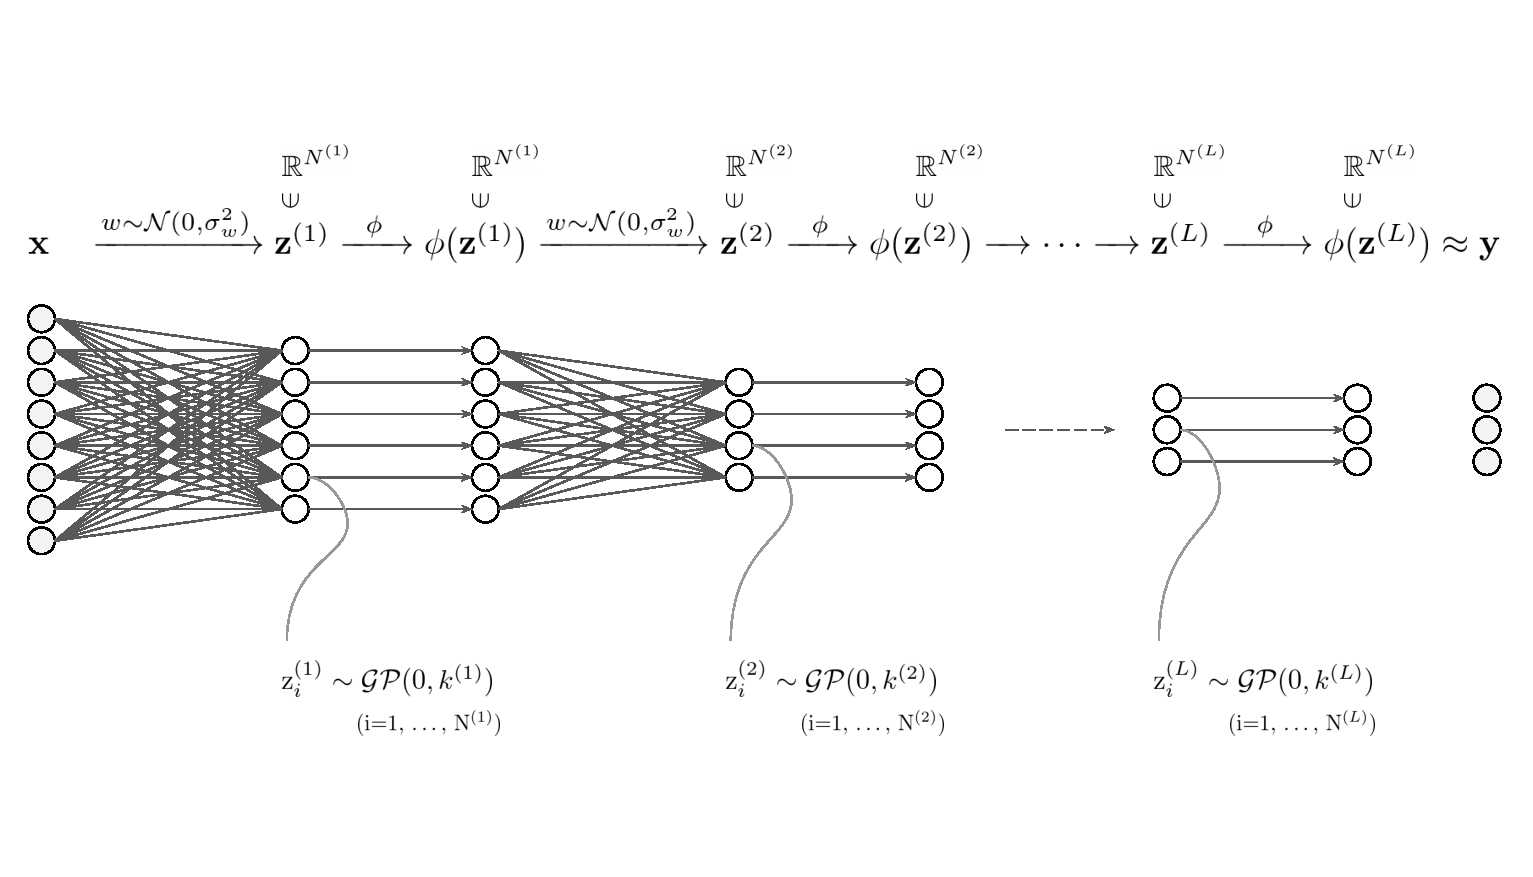
\includegraphics[width=12.0cm]{./figures/dnn_gp.eps}
            \caption{ガウス過程とDNN}
            \label{fig:dnn_gp}
          \end{center}
        \end{figure}
        上の議論から,任意の第$l$層に対して,カーネル関数$k^{(l)}$は次のように計算される.
        \begin{align}
          k^{(l)}({\bf x},{\bf x}') 
          &= Cov[ z_i^{(l)}({\bf x}), z_i^{(l)}({\bf x}')] \\
          &= E_w [z_i^{(l)}({\bf x}) z_i^{(l)}({\bf x}') ] \\
          &= E_w \left[ \left( \sum_{j=1}^{N^{(l-1)}} w_{ij} \phi(z_j^{(l-1)}({\bf x})) \right) \left( \sum_{j=1}^{N^{(l-1)}} w_{ij} \phi(z_j^{(l-1)}({\bf x}')) \right) \right] \\
          &= E_w \left[ \sum_{j=1}^{N^{(l-1)}} \sum_{k=1}^{N^{(l-1)}} w_{ij} w_{ik} \phi(z_j^{(l-1)}({\bf x})) \phi(z_k^{(l-1)}({\bf x}')) \right] \\
          &= \sum_{j=1}^{N^{(l-1)}} \sum_{k=1}^{N^{(l-1)}} E_w [w^2] \phi(z_j^{(l-1)}({\bf x})) \phi(z_k^{(l-1)}({\bf x}')) \\
          &= \sigma_w^2 \sum_{j=1}^{N^{(l-1)}} \sum_{k=1}^{N^{(l-1)}} \phi(z_j^{(l-1)}({\bf x})) \phi(z_k^{(l-1)}({\bf x}')) ~~~ ( l \geq 2 ) \\
          \\
          k^{(1)}({\bf x},{\bf x}') 
          &= Cov[ z_i^{(1)}({\bf x}), z_i^{(1)}({\bf x}')] \\
          &= E_w[z_i^{(1)}({\bf x}) z_i^{(1)}({\bf x}') ] \\
          &= \sigma_w^2 \sum_{j=1}^{N^{(1)}} \sum_{k=1}^{N^{(1)}} x_j {x'}_k 
        \end{align}
        さらに,任意の${\bf z}^{(l)} = {(z^{(l)}({\bf x}_1), \dots, z^{(l)}({\bf x}_N))}^{\mathrm{T} } \in \mathbb{R}^{N} $に対して,
        \begin{align}
          z^{(l)}({\bf x}_i) ~~ i.i.d. \sim p_z(\cdot), ~~~ E[z^{(l)}({\bf x}_i)] = 0, ~~~ (i=1, \dots, N)
        \end{align}
        を仮定すると,
        \begin{align}
          \phi ( z^{(l)}({\bf x}_i) ) ~~ i.i.d. \sim p_{\phi(z)}(\cdot), ~~~ E[\phi( z^{(l)}({\bf x}_i) )] = 0, ~~~ (i=1, \dots, N)
        \end{align}
        だから,
        \begin{align}
           & E_{{\bf x},{\bf x}'} \left[ k^{(l)}({\bf x},{\bf x}') \right] \\
          =& E_{{\bf x},{\bf x}'} \left[ \sigma_w^2 \sum_{j=1}^{N^{(l-1)}} \sum_{k=1}^{N^{(l-1)}} \phi(z_j^{(l-1)}({\bf x})) \phi(z_k^{(l-1)}({\bf x}')) \right] \\
          =& \sigma_w^2 E_{{\bf z}^{(l-1)},{{\bf z}'}^{(l-1)}} \left[ \sum_{j=1}^{N^{(l-1)}} \phi(z_i^{(l-1)}) \phi({z'}_i^{(l-1)}) \right] \\
          =& \sigma_w^2 E_{{\bf z}^{(l-1)},{{\bf z}'}^{(l-1)}} \left[ {{\boldsymbol \phi}({\bf z}^{(l-1)})}^{\mathrm{T}} {\boldsymbol \phi}({{\bf z}'}^{(l-1)}) \right] \\
          =& \sigma_w^2 N^{(l-1)} E_{z^{(l-1)},{z'}^{(l-1)} \sim \mathcal{GP}(0, k^{(l-1)})} \left[ \phi(z^{(l-1)}) \phi({z'}^{(l-1)})  \right] 
        \end{align}
        となることに注意する.

    \subsection{カーネル法}
      \subsubsection{正定値カーネルによる近似}
        式(\ref{form:nn_inference})の推論処理をまとめて関数$f_i:\mathbb{R}^{N} \to \mathbb{R}$とおく.
        \begin{align}
          y_i = f_i({\bf x}) = \phi( {{\bf w}_i}^{\mathrm{T}} {\bf x} )
        \end{align}
        ここで,関数$f_i$に対する内積${f_i(\cdot)}^{\mathrm{T}} f_i(\cdot): {\bf x} \times {\bf x}' \mapsto \mathbb{R}$を考える.
        活性化関数$\phi$としてReLUを仮定して,対応する指示 関数
        \begin{align}
          {\mathrm{I}}(x) = 
          \begin{cases}
            1 ~ (x \geq 0) \\
            0 ~ (x < 0)
          \end{cases}
        \end{align}
        を定義すると,
        \begin{align}
          {f_i({\bf x})} f_i({\bf x}') 
          &= {\mathrm{I}}( {\bf w}_{i}^{\mathrm{T}} {\bf x} ) {\mathrm{I}}( {\bf w}_{i}^{\mathrm{T}} {\bf x}' ) 
          ( {\bf w}_{i}^{\mathrm{T}} {\bf x} ) ( {\bf w}_{i}^{\mathrm{T}} {\bf x}' ) \\
          &= {\mathrm{I}}(\sum_{j=1}^{N} {w}_{ij} {x}_j) {\mathrm{I}}(\sum_{j=1}^{N} {w}_{ij} {x'}_j)
          ( \sum_{j=1}^{N} {w}_{ij} {x}_j ) ( \sum_{j=1}^{N} {w}_{ij} {x'}_j )          
        \end{align}
        となる.
        中心極限定理(Central Limit Theorem)より,任意の${\bf w} \in \mathbb{R}^{N}$の関数$C({\bf w})$に対して,
        \begin{align}
          E\left[ \frac{1}{M} \sum_{i=1}^{M} C({\bf w}_i) \right] \to
          \int d{\bf w} \frac{\exp (\frac{- {|| {\bf w} ||}^2}{2})}{{(2 \pi \sigma_w^2 )}^{N / 2}}
          C({\bf w}) ~~~ (M \to \infty)
        \end{align}
        が満たされるから,${\bf x}, {\bf x}'$を固定したとき,
        \begin{align}
          &E\left[ \frac{1}{M} \sum_{i=1}^{M} {f_i ({\bf x})} f_i ({\bf x}') \right] 
          = E\left[ \frac{1}{M} \sum_{i=1}^{M} {\mathrm{I}}( {\bf w}_{i}^{\mathrm{T}} {\bf x} ) {\mathrm{I}}( {\bf w}_{i}^{\mathrm{T}} {\bf x}' ) 
          ( {\bf w}_{i}^{\mathrm{T}} {\bf x} ) ( {\bf w}_{i}^{\mathrm{T}} {\bf x}' ) \right] \nonumber \\
          &\to \int d{\bf w} \frac{\exp (\frac{- {|| {\bf w} ||}^2}{2})}{{(2 \pi \sigma_w^2 )}^{N / 2}}
          {\mathrm{I}}( {\bf w}^{\mathrm{T}} {\bf x} ) {\mathrm{I}}( {\bf w}^{\mathrm{T}} {\bf x}' ) 
          ( {\bf w}^{\mathrm{T}} {\bf x} ) ( {\bf w}^{\mathrm{T}} {\bf x}' ) ~~~ (M \to \infty) \label{form:kernel_f} 
        \end{align}
        が成り立つ.式(\ref{form:kernel_f})右辺を整理すると,以下の定理が導かれる.

        \begin{dfn}
          (Arc-Cosine kernel)
          任意の2つのベクトル${\bf x}, {\bf x}' \in \mathcal{X} \subset \mathbb{R}^{N}$に対して,
          \begin{align}
            \theta &= {\cos}^{-1} \left( \frac{{\bf x}^{\mathrm{T}} {\bf x}'}{ \|{\bf x}\| \|{\bf x}'\| } \right) \\
            J(\theta) &= \sin \theta + (\pi - \theta) \cos \theta
          \end{align}
          とおき,Arc-Cosineカーネル
          \begin{align}
            k^{(1)}({\bf x}, {\bf x}') = \frac{1}{\pi} \| {\bf x} \| \| {\bf x}' \| J(\theta) 
          \end{align}
          を定義する.
        \end{dfn}

        \begin{thm}\label{thm:clt_dnn}
          各要素$w_{ij}$がi.i.d.で,平均が$0$,分散が$\sigma_w^2$となるランダム行列${\bf W} \in \mathbb{R}^{M \times N}$を考える.
          活性化関数としてReLU関数$\phi$を用いて,1層のニューラルネットワークに相当する関数$f_i:\mathbb{R}^{N} \to \mathbb{R}$:
          \begin{align}
            f_i({\bf x}) = \phi({\bf w}_i^{\mathrm{T}} {\bf x}), ~~~ (i=1 ,\dots, M)
          \end{align}
          を考える.このとき任意の${\bf x}, {\bf x}' \in \mathbb{R}^{N}$に対して,
          \begin{align}
            E \left[ \frac{1}{M} \sum_{i=1}^{M} f_i({\bf x}) f_i({\bf x}') \right] \to
            \frac{1}{\sigma_w^N} k^{(1)}({\bf x}, {\bf x}') ~~ (M \to \infty)
          \end{align}
          が成り立つ.
        \end{thm}

        \begin{thm}\label{thm:semi_positive}
          $\mathcal{X} \times \mathcal{X}$上の関数
          \begin{align}
            k^{(1)}({\bf x},{\bf x}') = \frac{1}{\pi} \| {\bf x} \| \| {\bf x}' \| J(\theta) \label{form:dnn_kernel}
          \end{align}
          は半正定値関数である.
        \end{thm}

        \begin{thm}\label{thm:kernel_matrix_positive}
          (カーネル関数存在定理)
          任意の対称行列$K \in \mathbb{R}^{n \times n} $が半正定値ならば,
          データ空間$\mathcal{X}$上の$n$点${ \{ {\bf x}_i \} }_{i=1}^{n}$と,
          特徴空間$\mathcal{F} \subset \mathbb{R}^{n}$上の$n$次元特徴ベクトル${ \{ f({\bf x}_i) \} }_{i=1}^{n}$がそれぞれ存在して,
          \begin{align}
            K_{ij} = {\langle f({\bf x}_i), f({\bf x}_j) \rangle}_{\mathcal{F}} = \sum_{k=1}^{n} {f({\bf x}_i)}_k {f({\bf x}_j)}_k 
          \end{align}
          が成り立つ.さらに,$k({\bf x}_i, {\bf x}_j) = K_{ij}$とおけば,半正定値関数$k: \mathcal{X} \times \mathcal{X} \to \mathbb{R}$が定義される.
        \end{thm}

        定理\ref{thm:kernel_matrix_positive}から,カーネル関数$k: \mathcal{X} \times \mathcal{X} \to \mathbb{R}$を定義せずとも,
        与えられたデータサンプルから構成された半正定値対称行列を作ることで,それが何らかのカーネル関数によるグラム行列に相当することが保証される.
        よって,定理\ref{thm:clt_dnn}と定理\ref{thm:semi_positive}より,式(\ref{form:dnn_kernel})を共分散関数にもつガウス過程が
        1層のNeuralNetworkの近似となることがわかる.

      \subsubsection{多層のFeed Forward Neural Network}
        1層のFeed Forward Neural Networkに関する議論は,正定値カーネルの線形性より,容易に多層へと拡張することができる.
        一般性を失うことなく,$L > 0$層からなるFeed Forward Neural Networkを考え,各層の線形写像に対応する重み行列${\bf W}^{(l)}$に対して,固定された$\sigma^2_w$を与えて,
        \begin{align}
          \forall l \in [1, L] \subset \mathbb{N}, ~~~ {\bf W}^{(l)}_{ij} \sim i.i.d. ~ \mathcal{N}(0, \sigma^2_w)
        \end{align}
        を仮定する.
        第$l$層のユニット数を$N^{(l)}$,第$l$層の空間を$\mathcal{T}^{(l)}$,第$l$層の出力を得る関数を$f^{(l)}: \mathcal{X} \to \mathcal{T}^{(l)}$とおく.
        任意の入力データ${\bf x}, {\bf x}' \in \mathcal{X}$に対して,Neural Networkの第$l$層に対応する共分散関数$k^{(l)}: \mathcal{T}^{(l)} \times \mathcal{T}^{(l)} \to \mathbb{R}$は,次の漸化式で求められる.
        \begin{align}
          k^{(1)}({\bf x}, {\bf x}') &= Cov \left[ f^{(1)}({\bf x}), f^{(1)}({\bf x}') \right] \nonumber \\
                                    &= Cov \left[ \phi({\bf W}^{(1)} {\bf x}), \phi({\bf W}^{(1)} {\bf x}') \right] \nonumber \\ 
                                    &= \frac{1}{\pi \sigma_w^{N^{(1)}}} \| {\bf x} \| \| {\bf x}' \| J(\theta^{(0)}) \\
          k^{(l+1)}({\bf x}, {\bf x}') &= Cov \left[ f^{(l+1)}({\bf x}), f^{(l+1)}({\bf x}') \right] \nonumber \\
                                      &= Cov \left[ \phi( {\bf W}^{(l+1)} \cdots \phi( {\bf W}^{(1)} {\bf x} )), \phi( {\bf W}^{(l+1)} \cdots \phi( {\bf W}^{(1)} {\bf x}' )) \right] \nonumber \\ 
                                      &= \frac{1}{ \pi \sigma_{w}^{ N^{(l+1)}}} \sqrt{ k^{(l)}({\bf x}, {\bf x}) } \sqrt{ k^{(l)}({\bf x}', {\bf x}') } J(\theta^{(l)})
        \end{align}
        ただし,
        \begin{align}
          J(\theta^{(l)}) &= \sin \theta^{(l)} + (\pi - \theta^{(l)}) \cos \theta^{(l)} \\
          \theta^{(l)} &=
          \begin{cases}
            \cos^{-1} \left( \frac{{\bf x}^{\mathrm{T}} {\bf x}'}{ \|{\bf x}\| \|{\bf x}'\| } \right) ~~~ (l = 0) \\
            \cos^{-1} \left( \frac{k^{(l)}( {\bf x}, {\bf x}' )}{ \sqrt{ k^{(l)}({\bf x}, {\bf x}) } \sqrt{ k^{(l)}({\bf x}', {\bf x}') } } \right) ~~~ (l \neq 0) 
          \end{cases}
        \end{align}
        とする.以上の結果から,入力から第$l$層の各ユニットの出力値を得る関数$f^{(l)}_i: \mathcal{X} \to \mathbb{R}$は以下のガウス過程で近似できる.
        \begin{align}
          f^{(l)}_i(\cdot) \sim \mathcal{GP}( 0, k^{(l)}(\cdot,\cdot) ), ~~~ (i=1,\dots,N^{(l)})
        \end{align}

  \section{Kernel Variational AutoEncoder}
    前章での議論から,GP-LVMにおける潜在変数$X$と観測関数$Y$に対する確率モデル$p(Y|X)$を,
    多層のFeed Forward Neural Networkに相当するモデル
    \begin{align}
      y = f^{(l)} ({\bf x}) = \phi( {{\bf w}^{(l)}}^{\mathrm{T}} \phi( {\bf W}^{(l-1)}  \dots \phi( {\bf W}^{(1)} {\bf x}) ) )
    \end{align}
    によって表現することを考える.すなわち,
    \begin{align}
      k^{(l)}( {\bf x}, {\bf x}' ) = { \langle f^{(l)} ({\bf x}), f^{(l)} ({\bf x}') \rangle }_{\mathcal{F}^{(l)}}
    \end{align}
    に対応するガウス過程
    \begin{align}
      f^{(l)}(\cdot) \sim \mathcal{GP}(0, k^{(l)}(\cdot,\cdot))
    \end{align}
    を考える.

    \subsection{変分推論}

  \section{Experiments}
  \section{Conclusion}
    文献\cite{Hinton1995BayesianLF}
    \cite{DLGP2018} \cite{KMDL2009} \cite{LawrenceGPLVM2004} \cite{LawrenceGPLVM2005}
    \cite{SparseGP2006} \cite{VariationalSparseGP2009} \cite{BayesGP2010}
    \cite{GPBIGDATA2013}


  \bibliography{ref} %hoge.bibから拡張子を外した名前
  \bibliographystyle{junsrt} %参考文献出力スタイル
  
\end{document}